\documentclass{article}
\usepackage{geometry}[a4paper, margin=2in]
\usepackage{graphicx}
\usepackage{float}
\usepackage{subfigure}
\title{Practical Submission Sheet}
\newcommand{\bb}[1]{\textbf{#1}}
\date{}
\begin{document}
	\maketitle
	\begin{tabular}{ll}
		\bb{Term}: 2020-1 & \bb{Submission Date}: \today\\
		\bb{Lecture Date}: August 21, 2020. & \bb{Practical Number}: 3\\
		\bb{Course Code}: PHY249 & \bb{Section}: G2903\\
		\bb{Registration Number}: 11912610 & \bb{Roll No}: 03\\
		\bb{Student Name}: Aayush Arya & \\
	\end{tabular}
	
	\section*{Concepts Learnt}
	Learnt how a transistor circuit can be configured to provide a logical output, specifically as a NOT gate. Gained a physical understanding of how the circuit behaves.
	
	\section*{Key Observations \& Insights}
	The circuit behaves as a logical NOT gate. It is due to the feature that a transistor as a whole acts as two separately configurable pn junctions. Logical and analog DC inputs are equivalent when the concern is merely the output.
	
	\section*{Application Areas}
	Transistors can as logic gates and switches which need not to be toggled manually and are thus useful in electronic devices ranging from computers to mobile phones.
	\section*{Report}
	An $npn$ transistor circuit was created in common emitter configuration. In this configuration, the emitter is grounded, the base acts as an input terminal and the collector as an output. Initially, a logical input source was used, as shown in figure 1. \\
	
	A transistor has two $pn$ junctions. One pn junction is forward biased and the other is reverse biased. In our case, when the logical input is in "high" mode, it is equivalent to the base (which is of p-type material) being connected to a positive terminal. The emitter is connected to the negative terminal of a DC supply, thus making the base-emitter junction forward biased. Thus, in the case when the input to the base is "high",the current flows from the base through the emitter to the negative terminal of the battery which is rated 5V. Then, most of the $5V$ is lost as potential drop across the $100\Omega$ resistor and thus the potential drop across the terminals of the LED goes down to a very small value. Consequently, the LED doesn't glow.


	\begin{figure}[H]
	\begin{center}
		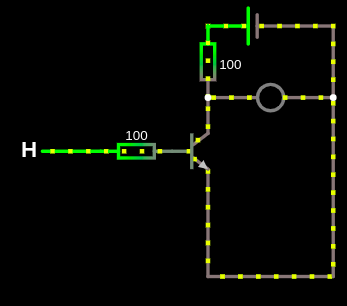
\includegraphics[width=0.6\textwidth]{NOT_gate.png}
		\caption{The simulator circuit diagram of the NOT gate formed using a transistor.}
	\end{center}
\end{figure}

	When the input to the base is in the "low" state, the base is as if connected to a negative terminal and the collector (n-type) is already connected to the postive terminal of a battery. Thus, the collector-base junction acts as if it's reverse biased and no current flows through the transistor. The entire current now passes through the $100\Omega$ resistor and LED which now glows.\\
	
	A similar effect can be obtained using a DC supply as the input instead of a logical input, as shown in Figure 2.

\begin{figure}[H]
	\begin{center}
		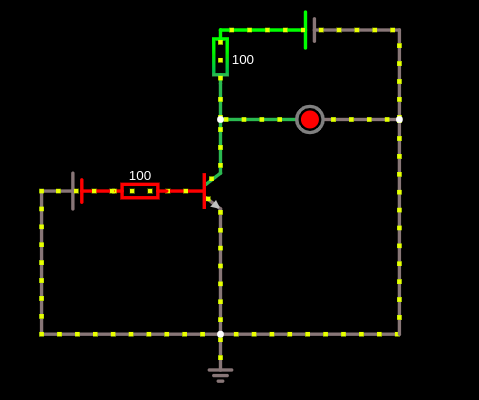
\includegraphics[width=0.6\textwidth]{DC_input.png}
		\caption{If the base terminal of the transistor is connected to a DC supply, it behaves as a switch.}
	\end{center}
\end{figure}



\end{document}